\chapter{SynVisio}

Our biggest contribution in this research was the development of SynVisio an online platform to explore syteny by mapping syntenic blocks that are highly conserved and long enough to be significant between a given pair of genomes or within a single genome.In this chapter we first discuss the different modes SynVisio offers for synteny analysis and how each one operates.We then explore the different features SynVisio provides to enhance user experience with the tool.Following this we discuss the software implementation of the tool and the elaborate on choices made regarding its web architecture.Finally we look at a basic usage scenario through a series of steps depicting how SynVisio can be used to explore the genomic conservation between a sample data-set of humans and chimpanzees.

\section{System Overview}
SynVisio is a multi scale genome browser that can be accessed through the web and lets researchers explore genomic conservation.It lets researchers upload output files of synteny detection system of their choice and generates visualizations on demand from the information in these files.It offers two analysis modes : Single Level and Multi Level.In the first mode users can compare genomes two at a time through a dashboard where syteny is visualized as both a dot plot and a linked parallel plot.The charts are accompanied by a filter panel where the conserved genomic blocks can be filtered based on features such as the degree of similarity.In the second mode researchers can compare several genomes at a time through multi level representations such as hive plots and stacked parallel plots.To aid researchers in their visual exploration of synteny,SynVisio lets them annotate the generated charts with additional tracks in the form of histograms, heat-maps and other basic plots.Additional features are also provided such as a gene search panel to look for specific genes by gene ID and the ability to export generated charts for publication.


\section{Analysis Mode}
Gene sequences can be compared in different ways depending on the underlying biological question.Which means syteny analysis can vary between visualizing simple pairwise matches between two genomes to preforming multi way comparisons across several genomes at once.The availability of datasets and their inherent quality also plays into the kind of analysis that can be done.Whole genome alignment for example is usually done pairwise as looking for matches can be faster when the subset of available matches is low.Additionally in the context of Synteny detection which is anchor   based, identifying common markers between multiple genomes is difficult\cite{wang2012mcscanx}.However when the data is available, multi way comparisons can offer better insights and tackle bigger questions like pan genome syteny.Thus SynVisio offers both a Single and a Multi Level analysis mode depending on the the researchers choice and the availability of data.

\subsection{Single Level Analysis}
This is default mode in which SynVisio operates and is meant for exploratory tasks as it presents the collinearity between a selected set of chromosomes in two different visual representations and lets users filter the collinear blocks on the fly.Although our system operates as dashboard with multiple representations in coordinated views we offer users the ability to  look only at one particular representation through the configuration page.This is meant to make our system unopinionated in the choice of representation and lets users make the decision on how they want their data visualized. 

\begin{figure}
  \centering
  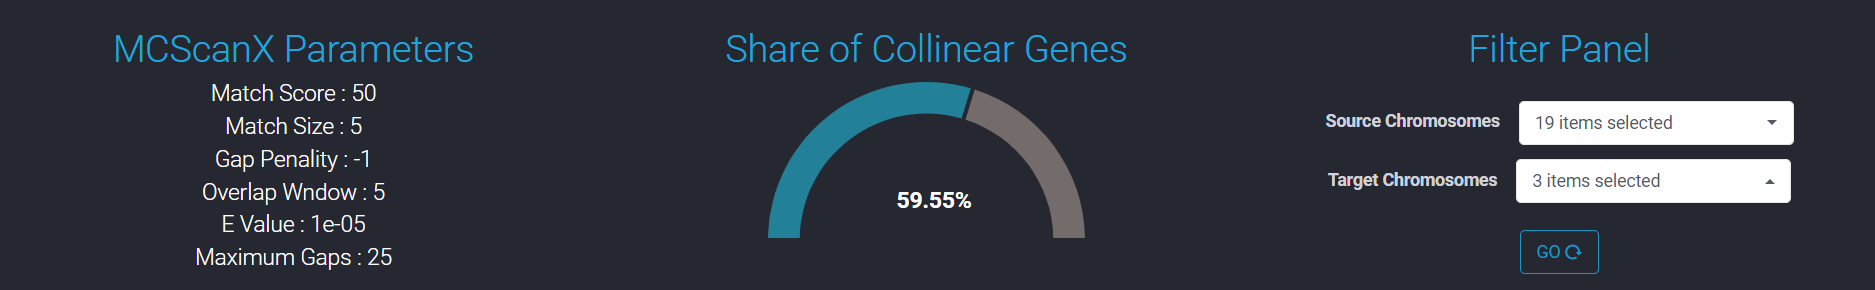
\includegraphics[width=1\linewidth]{images/ch_5_baseparameters.PNG}
  \captionof{figure}{Synteny detection parameters and level of collinearity presented along with toggles to select source and target chromosomes.}
  \label{fig:ch_5_baseparameters}
\end{figure}


The first step involved in using the dashboard is providing an input dataset, for this, users can either upload their own datasets or use existing sample files.We have already processed several datasets depicting genome conservation on a wide range of species.These are available on the homepage of our application and are updated on a monthly basis.Some of the examples include self syteny in Brassica napus(canola), cross syteny between Oriza satica(rice) and Sorghum bicolor(broom-corn) and cross syteny between Arabidopsis thaliana(thale cress) and Vitis vinifera(grape vine).After the initial data uploading and processing stage is complete basic information about the parameters used in the syteny detection process are presented along with the percentage share of collinearity present in the files accompanied with toggles to select the source and target chromosomes as shown in Figure \ref{fig:ch_5_baseparameters}.If outputs of synteny detection systems other than MCScanX are uploaded the parameters tab and the percentage share of collinear genes chart are left blank . The list of chromosomes are ordered alpha-numerically to divide the different species into distinct groups and make it easier to pick chromosomes sequentially.Additional buttons are also provided to either``Select All" or ``Clear All" in both the drop-drown lists intended for picking chromosomes.


When a user hits the button ``GO" to get started the first visualization presented at the top is a parallel link plot where syntenic collinear blocks are connected by coloured ribbons as shown in Figure \ref{fig:ch_4_dashboard}.The source chromosomes are laid out on the top and the target chromosomes are spread out in the bottom.The size of the chromosomes are calculated based on the genomic sizes of the chromosomes and the available screen width to ensure that the visualizations are responsive across different screen-sizes.Chromosomes in the source layer are coloured using a chromatic 10 point color scale derived from ColorBrewer\cite{colorbrewer} and are set to repeat after every 10 chromosomes as humans can find it hard to perceive differences beyond a dozen colours\cite{ware2012information}.The connecting ribbons represent collinear blocks with the colour of a ribbon representing its source chromosome.The connecting ribbons can have varying widths at either ends due to the size of the collinear block they represent. Although collinear blocks have the same gene count at either side the width of the block in terms of base pairs can be quite different at either sides due to variable gap sizes between individual genes.This scaled representation of connected ribbons can also mean that certain ribbons can end up being smaller than a single pixel in width due to their small genomic size.So we clamp our scale at the lower end to 2 pixels to ensure that extremely small ribbons are still represented as 2 pixel wide lines instead of ribbons.

While the parallel link chart is designed to take half of the available vertical space, the other half is made up of a dot plot and an adaptive filter panel consisting of a scatter plot.The dot plot as explained in the visual design chapter uses positional encoding and represents collinear blocks as either dots or lines.To ensure that extremely small collinear blocks are still represented on the screen we limit them to single pixel wide dots on the chart while larger blocks are encoded as lines.The dot plot works in coordinated manner with the parallel link plot and so any actions in one are also reflected in the other as shown in figure {cite linking view}. Since the dot plot is always meant to be square it has a fixed aspect ratio and thus the filter panel expands to fill the remaining horizontal space.It provides filtering through three parameters : Gene count, Match Score and E(expect) value.It is set to filter using gene count by default but can be changed using the radio buttons provided to the left.To offers users context into the parameter being filtered its value for all the collinear gene blocks are visualized as a simple scatter plot.Every collinear gene block is represented by a single dot irrespective of its size  and is colour coded to correspond to the chromosomes in the parallel plot.The scale of the plot is adaptive and automatically changes based on the parameter in question.Gene count and Match Score correspond to the number of genes in a collinear block and the alignment score assigned to that block respectively and are represented in a linear scale.E-value or expect value is the measure of probability that a match has occurred by chance and owing to the wide range in which this value can be reported it is represented in a logarithmic scale.Researchers can use the slider to control the visibility of collinear blocks they see in the other two views.The position of the slider on the chart is represented with a dashed line that is annotated with the value at which the charts are currently being filtered.

\begin{figure}
  \centering
  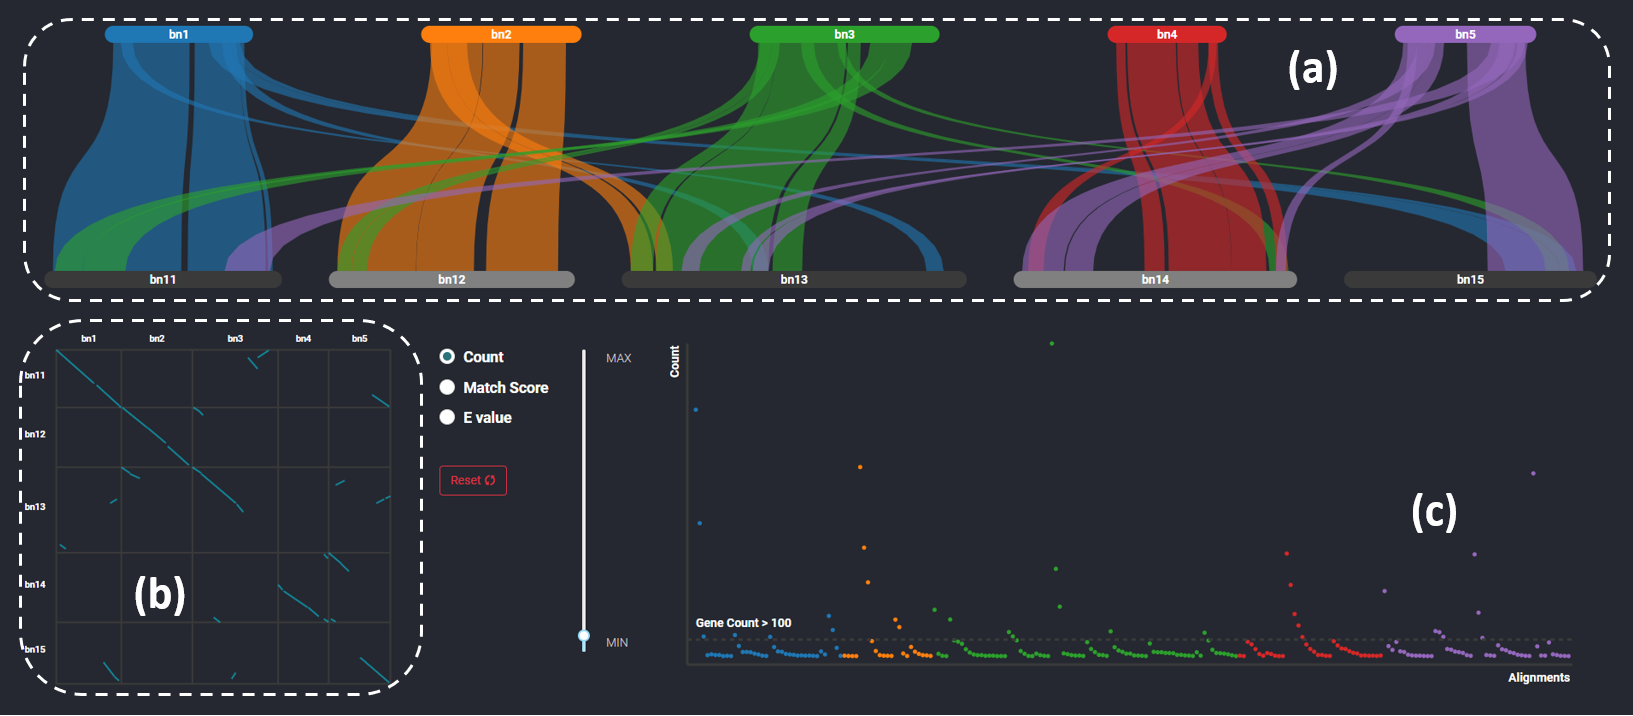
\includegraphics[width=.75\linewidth]{images/ch_1_dashboard.PNG}
  \captionof{figure}{Single analysis mode visualizing genome collinearity in Bn(Brassica Napus) with the following components: \textbf{a)} Parallel Link Plot \textbf{b)}Dot plot and \textbf{c)} Filter panel}
  \label{fig:ch_4_dashboard}
\end{figure}


% For uploading their own datasets users need to provide two files, a collinearity file that is generated using a syteny detection software like MCScanX or DAGChainer containing the list of collinear blocks and a GFF file for the positions of all the reference genes in the genome.


% In this Mode SynVisio operates as a dashboard by default and presents genome collinearity in multiple representations.Users however have the choice to switch the visual representation using the configuration page and options available are a dot plot,a linear connector plot, and an exploratory dashboard with both plots and a filter panel.


% First talk about parameters and overall percentage share between source and target. and why its shown
% then filter panel why we select chromesome differe source and target. why they are sorted apla nuerically

% then we talk about the linear link plot then dot plot.
% then the filter panel why we need it..why the different features. why the slider. choice of colours at this stage.

% then chromosome mode .different colour for inversions then the ability to zoom and hover over links to see what they contain.

% then individual block mode then invert entire chromosome. then shift axis to right or zoom.



\subsection{Multi Level Analysis}
Hive Plots and Stacked Bar plots

\section{Usability Features}
\subsection{Track Annotation}
\subsection{Re-visitation Support}
\subsection{Gene Search Panel}
\subsection{Image Export}


\section{Usage Scenario}
A series of pictures explaining a particular exploratory scenario - Best done with Wheat genome showing genome triplication and further interlocation of some chromosomes.